\section{Methods}
This chapter covers the methodology used to conduct the experiment which is the main focus of this paper.
It will cover the research design, the experiment setup and execution, as well as the data transformation 
and visualisation.\\

\subsection{Research Design}
The research of this paper is based on empirical and quantitative data collected from an experiment.
The experiment is made up of the following variables, the independent variable, the number of training iterations the
program is trained with, and the dependent variable, the accuracy of the model. To make sure results are accurate and consistent, 
all iterations will use the same machine learning algorithm,
the same dataset, the same evaluation data, and run on the same hardware.
The data which is being collected and analyzed is the number of iterations (categorical ordinal), the accuracy
and loss (continuous ratio), and the relation between them.\\

\begin{table}[h]
\centering
\begin{tabularx}{\textwidth}{|>{\hsize=.5\hsize}X|>{\hsize=1.5\hsize}X|}
\hline
\textbf{Type} & \textbf{Variable} \\
\hline
Independent Variable & 
\begin{tabular}{@{}l@{}}
\textbullet{} Number of Iterations  \\
\end{tabular} 
\\
\hline
Dependent Variable & 
\begin{tabular}{@{}l@{}}
\textbullet{} Accuracy of the Model\\
\end{tabular} 
\\
\hline
Controlled Variable & 
\begin{tabular}{@{}l@{}}
\textbullet{} Machine Learning Algorithm \\
\textbullet{} Dataset, Evaluation Data \\
\textbullet{} Hardware \\
\end{tabular} 
\\
\hline
\end{tabularx}
\caption{Key Variables of the Experiment}
\label{table:1}
\end{table}

\subsection{Experiment Setup and Execution}
The program "CreateML" from \cite{Apple} was used to carry out this experiment. It is a user-friendly and powerful 
tool that allows developers to create custom machine-learning models without the need for extensive expertise in the field.
CreateML simplified the process of creating and training an object detection model by providing a graphical user interface which 
just takes the input dataset and the desired parameters. The object detection model uses the YOLOv2 \parencite{Jaina} algorithm.
"You Only Look Once" (YOLO) is a state-of-the-art, real-time object detection algorithm introduced in 2015" \parencite{Keita2022}. 
The dataset used to train the object detection model is \citetitle{pascal2023} which is a collection of around 10000 images including classes
like persons, vehicles and animals. The experiment was run on a MacBook Air 2020 with an Apple M1 chip and 8GB of RAM. To ensure the 
result were unbaised the "Batch Size" was left on auto and the "Grid Size" was set to 13x13.\\

\newpage
Overall the model was trained 20.000 times and every 1000 iterations a snapshot of the model was taken and evaluated using
specific images. 
The classes and images chosen include: Boat, Dog, Person, Plant, Wheel (See Appendix~\ref{app:test-pictures}).
\begin{figure}[h]
  \centering
  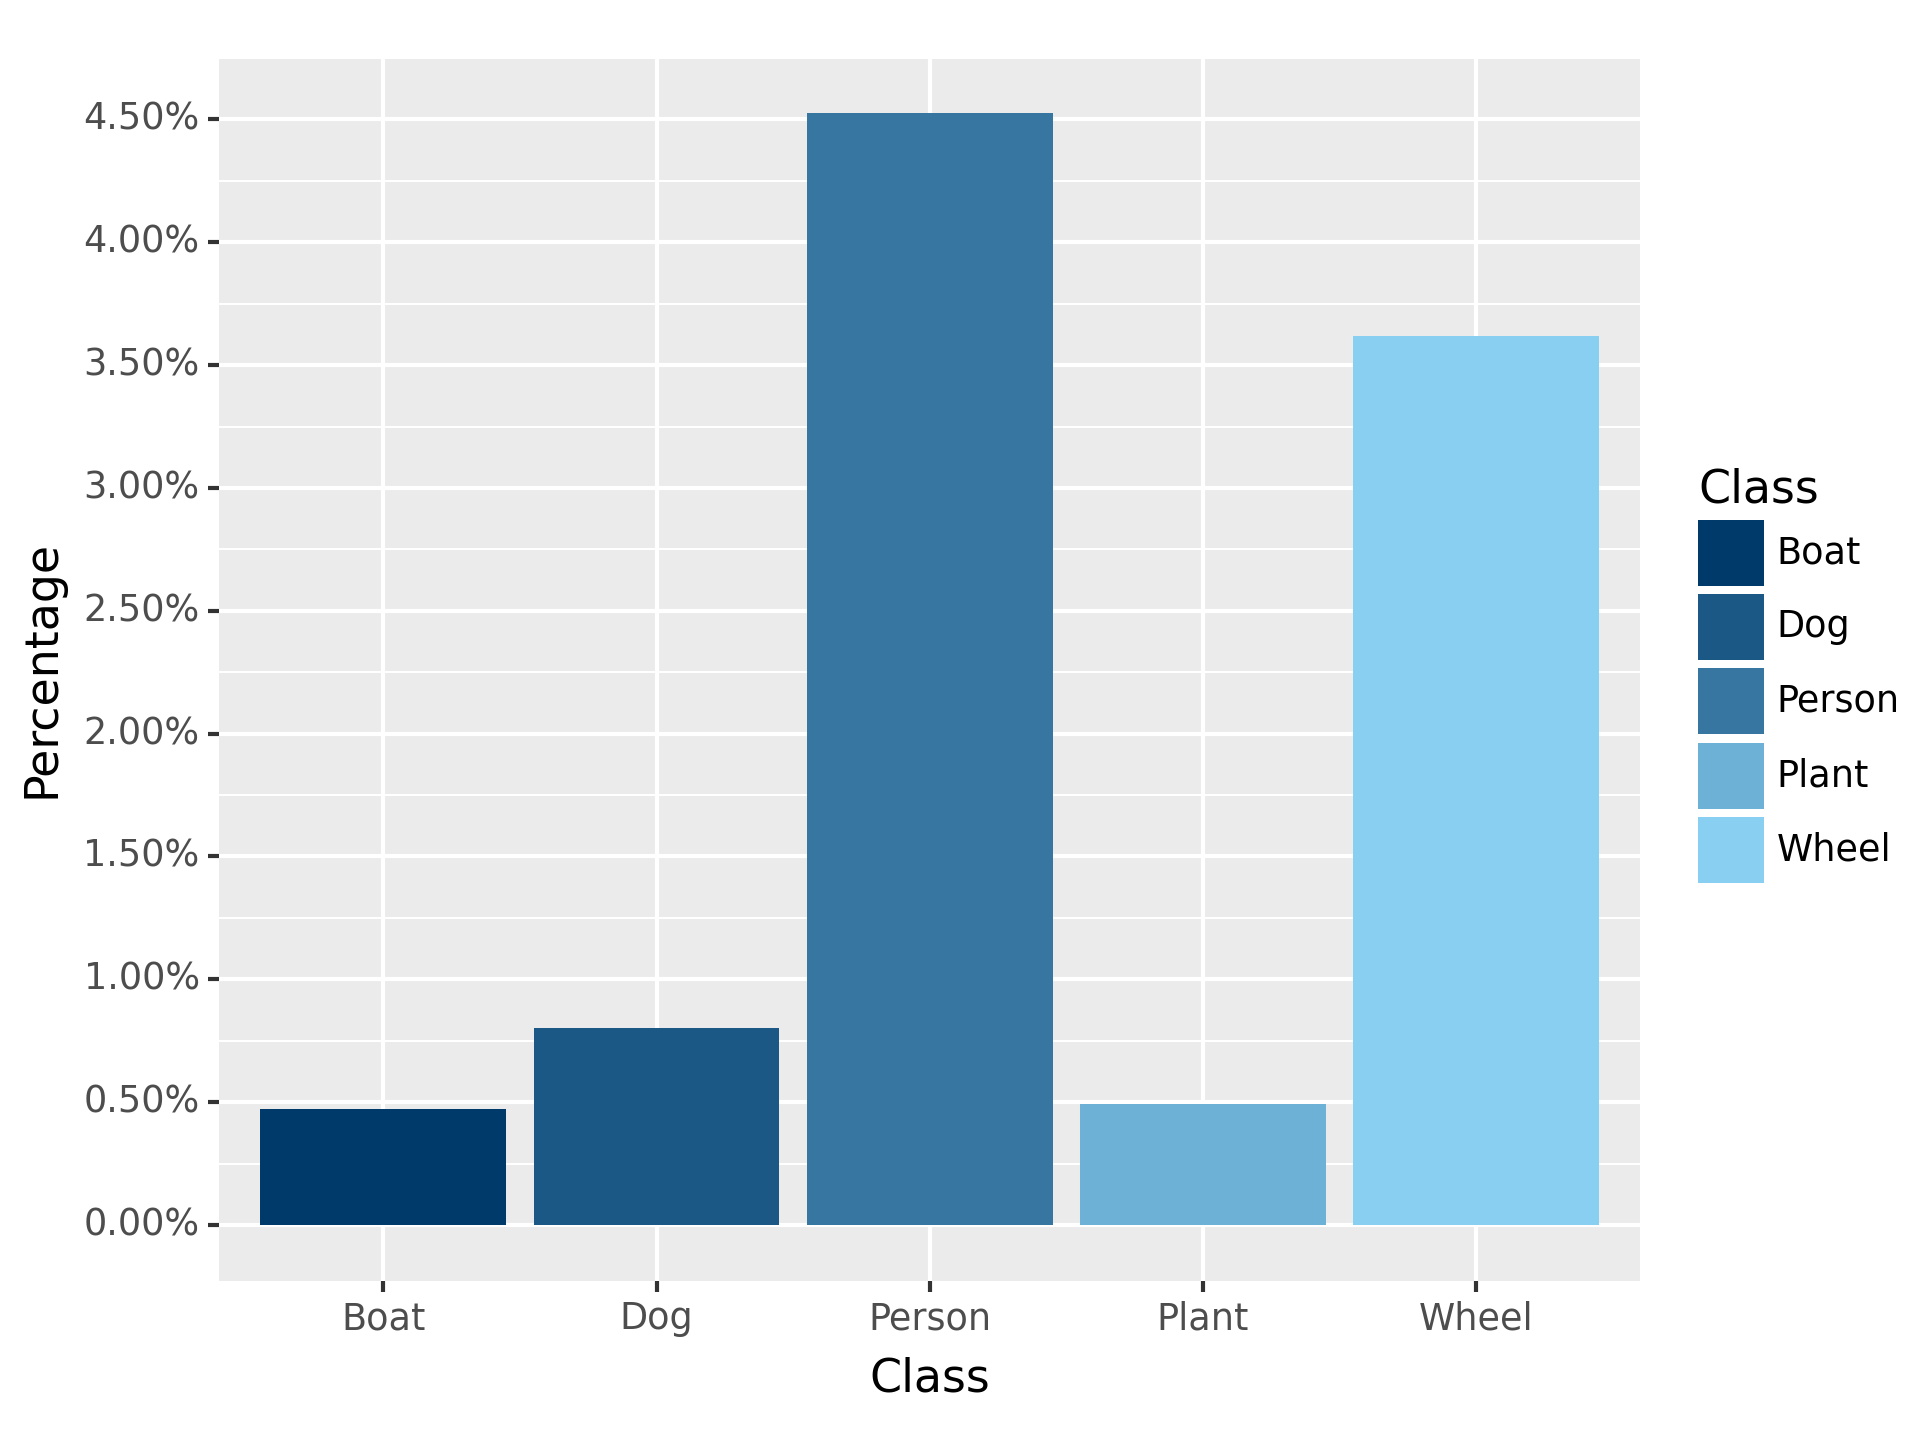
\includegraphics[width=0.70\textwidth]{../Data/distribution-classes-barchart.png}
  \caption{Class Usage in Dataset (\%)}
  \label{fig:class-usage-in-dataset}
\end{figure}
\\
Each snapshot was evaluated by using the above-mentioned images and the accuracy as well as the loss was saved in a CSV file for 
analysation.
\\
\subsection{Data Transformation and Visualisation}
Data transformation and its visualisation plays a crucial role in evaluating the hypothesis. The gathered data was exported to multiple CSV files, 
which were categorized by class and consisted of the number of iterations and the accuracy per picture. Python and Jupyter Notebooks were the
foundation for the handling of data in this project. Data manipulation was handled by Pandas and the visualisation was done using Matplotlib
and Plotnine.\\

% CLASS DISTRIBUTION
The annotations JSON file, included in the training dataset \parencite{pascal2023}, was an additional source of information. 
A custom Python script was written to transform the data into a useable format, which was required to calculate the class distribution 
and the image count per class. To illustrate which classes were evaluated and their representation in the dataset, a bar chart was created 
(See Fig.~\ref{fig:class-usage-in-dataset}). This choice was motivated by the observation that "[v]ertical bar charts are useful to compare 
different categorical [...] variables" \parencite{Statistics-Canada2021}.\\ 
\newpage

% LOSS GRAPH
The loss was graphed by using a scatter plot (See Fig.~\ref{fig:loss-vs-training-iterations})
as it visualises the relationship between two or more quantitative variables. They are especially helpful when examining whether
the values of one variable are influenced by the values of the other variable \parencite{Statistics-Canada2021b}. 
Additionally, a quadratic trend line was added to identify the trend and outliers.\\ 

% ACCURACY GRAPH
To plot the accuracy all CSV files were merged by iterating through each file, calculating the mean accuracy per iteration and appending it
to the new pandas data frame. This resulted in a data frame with the mean accuracy per iteration for each class. This data was then plotted using
a line chart (See Fig.~\ref{fig:accuracy-vs-training-iterations}). \\ 

% ACCURACY IMPROVEMENT GRAPH
To illustrate the improvement of accuracy over time, the average accuracy of all classes per iteration was calculated.
From that, the percentual increase of accuracy was calculated and then the average accuracy was plotted against the number of iterations
(See Fig.~\ref{fig:accuracy-improvement}).
A line chart was chosen for both because it is useful for illustrating trends over time \parencite{Statistics-Canada2021a}.\\

% BAR CHART FLUCTUATION WHEEL AND DOG
For further investigation into the performance of some classes, the accuracy for a specific iteration per picture was plotted 
using a line and bar chart (See Fig.~\ref{fig:14000-dog}, \ref{fig:image-1-accuracy}, \ref{fig:13000-wheel}, \ref{fig:image-3-accuracy}). 
This was done to identify outliers and to clearly display discrepancies in performance between pictures of the same class.\\

% BOX PLOT PER ITERATION
To obtain a comprehensive insight into the variation in the model's accuracies, a box plot was utilised (See. Fig~\ref{fig:Box-plot}). This visual representation illustrated the distribution of the accuracy measurements gathered during the experiment, portraying how the model evolved throughout its training process.
This graph is a good choice since its use case is illustrating the distribution of data \parencite{Tableau}.\\

